\documentclass{article}
\usepackage{fancyhdr,amssymb,amsmath,amsthm,bbm,enumerate,mdwlist,url,multirow,hyperref,graphicx,dsfont}
\usepackage{pdfpages}
\usepackage{algorithm}
\usepackage{algpseudocode}
\addtolength{\hoffset}{-1.5cm}
\addtolength{\textwidth}{3cm}
\addtolength{\voffset}{-1.5cm}
\addtolength{\textheight}{3cm}


\usepackage[slovene]{babel}
 \usepackage[utf8]{inputenc}
\usepackage[T1]{fontenc}
\usepackage{graphicx}


\begin{document}
\newtheorem{definition}{Definicija}


\title{Graphs of type (SB) and domination on their cartesian products}

\author{Jan Hrastnik, Matic Kremžar}
\date{11. 12. 2024}
\maketitle


\section{Uvod}
V projektni nalogi sva se ukvarjala z grafi tipa (SB) in dominacijo na njihovem kartezičnem produktu. 
Projektna naloga je bila izvedena v programu SageMath, obsežni izračuni pa s pomočjo spletne strani CoCalc, in predvsem lokalno na Linux-u.
Naloga ima odprt tudi svoj repozitorij na GitHubu, na naslovu \href{https://github.com/matickremzar/Graphs-of-type-SB-and-domination-on-their-cartesian-products-/tree/main}{(tukaj)}.
Tam so zbrane tudi vse datoteke, ki sva jih uporabila med izdelavo projekta.

Cilj je razumeti, kako prepoznati, konstruirati in spreminjati grafe tipa (SB), 
ter analizirati njihove lastnosti, zlasti dominacijsko število njihovih kartezičnih produktov.

\section{Osnovna ideja in definicije}
Delala sva z usmerjenimi grafi $G = (V,E)$, kjer je $V$ množica vozlišč, $E$ 
pa množica povezav grafa.

\begin{definition}
    Graf $G$ je tipa $(SB)$, če je njegov premer enak $2$ in ima dve sosednji vozlišči $v_1, v_2\in V$, da velja:
    \begin{itemize}
        \item $v_1$ in $v_2$ nimata skupnega soseda,
        \item $G$ ima vozlišče $v^*\in V$, ki ni sosednje $v_1$ ali $v_2$; torej $v^*\not\sim v_1$ in $v^*\not\sim v_2$. \newline
    \end{itemize}
\end{definition} 

\begin{figure}[h!]
    \centering
    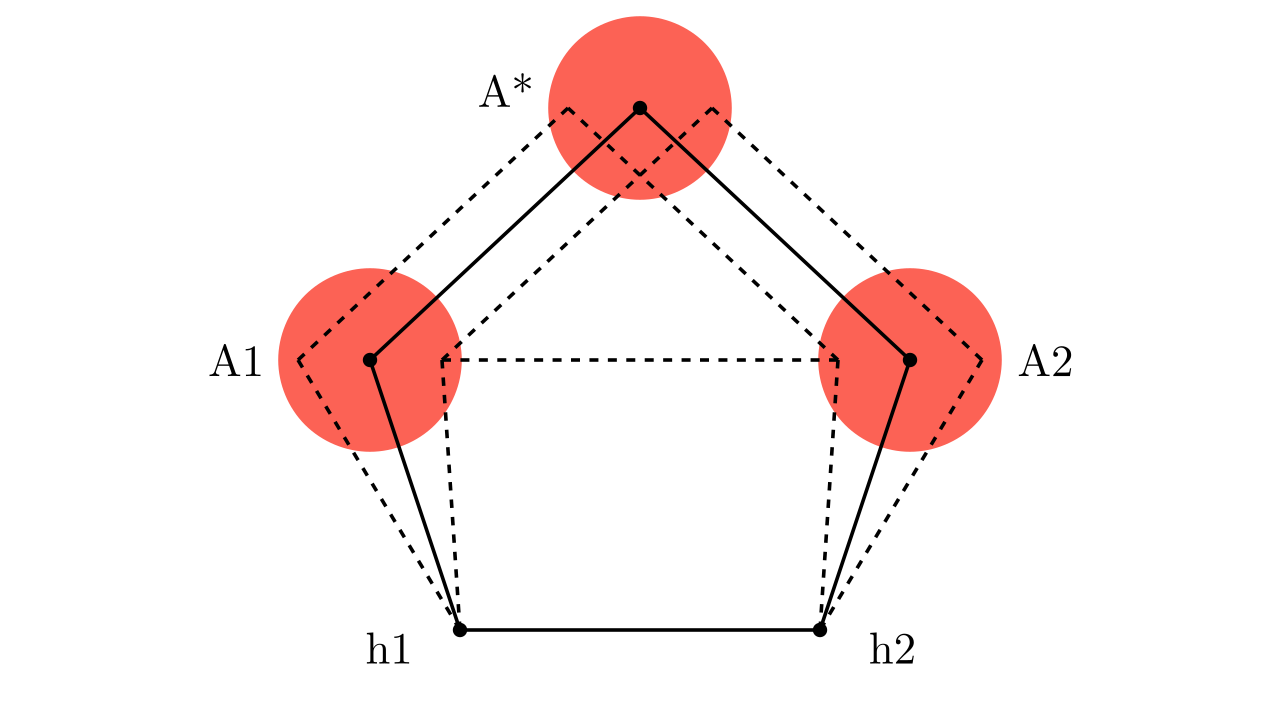
\includegraphics[width=0.5\textwidth]{GraphPlanarDegrees_ManimCE_v0.18.1.png} % 0.5 pomeni pol širine strani
    \caption{Skica grafov tipa (SB)}
    
\end{figure}

Zapišemo lahko particijo vozlišč grafa $G$ kot $$V(G) = {v_1, v_2} \cup A_1 \cup A_2 \cup A^*,$$
kjer je $A_1$ množica vozlišč, ki so sosednja $v_1$, $A_2$ množica vozlišč, ki so sosednja $v_2$ in 
$A^*$ množica vozlišč, ki niso sosednja niti $v_1$ niti $v_2$.

\begin{definition}
   Podmnožica vozlišč $D\subseteq V$ grafa $G=(V,E)$ se imenuje \emph{dominacijska množica} grafa,
   če je vsako vozlišče $v\in V$ grafa v množici $D$, ali pa je kakšno njemu sosednje vozlišče
   v $D$. \emph{Dominacijsko število $\gamma(G)$} grafa je velikost najmanjše dominacijske
   množice grafa.
\end{definition}

\begin{definition}
    Kartezični produkt $G\square H$ grafov $G$ in $H$ je graf, za katerega velja:
    \begin{itemize}
        \item vozlišča grafa $G\square H$ so kartezični produkt $V(G)\times V(H)$,
        \item dve vozlišči $(u,v)$ in $(u',v')$ sta sosednji v grafu $G\square H$ natanko tedaj, ko je:
        \begin{itemize}
            \item $u=u'$ in $v$ je sosed $v'$ v $H$, \textbf{ali}
            \item $v=v'$ in $u$ je sosed $u'$ v $G$.
        \end{itemize}
    \end{itemize}
\end{definition}

\section{Naloga 1}
\subsection{Preverjanje, ali je graf tipa (SB)}
Sprva je potrebno zapisati kodo, ki preveri, ali je dan graf tipa (SB) (v datoteki $sb\_detect\_koncna.py$). Uporabimo matriko sosednosti. Dovolj je, 
da pregledamo zgolj zgornji trikotnik matrike, saj tako že pridobimo vse podatke o sosedih. Nato 
preverimo še veljavnost prej zapisanih lastnosti grafov tipa (SB). Najina metoda za preverjanje, ali je graf tipa (SB), ima časovno zahtevnost $O(|V|^3)$.



\begin{algorithm}
\caption{Preverjanje, ali je graf tipa (SB)}
\begin{algorithmic}[1]
\Function{IsSB}{G: Graph} \Comment{Funkcija za preverjanje grafa tipa (SB)}
    \State \textbf{if} $G.diameter() \neq 2$ \textbf{then} \Return \textbf{False} \Comment{Premer mora biti 2}
    \State $adj \gets G.adjacency\_matrix()$ \Comment{Pridobimo matriko sosednosti}

    \For{$i \gets 1$ \textbf{to} $adj.nrows()$}
        \For{$j \gets i+1$ \textbf{to} $adj.nrows()$} \Comment{Samo zgornji trikotnik}
            \If{$adj[i, j] = 1$} \Comment{Če sta $i$ in $j$ soseda}
                \State $common\_neighbour \gets \textbf{False}$
                \For{$k \gets 1$ \textbf{to} $adj.nrows()$}
                    \If{$adj[i, k] = 1$ \textbf{and} $adj[j, k] = 1$} \Comment{Preverimo skupne sosede}
                        \State $common\_neighbour \gets \textbf{True}$
                        \State \textbf{break}
                    \EndIf
                \EndFor
                \If{$common\_neighbour$}
                    \State \textbf{continue}
                \EndIf

                \State $nonadj\_vertex\_exists \gets \textbf{False}$
                \For{$k \gets 1$ \textbf{to} $adj.nrows()$}
                    \If{$adj[i, k] = 0$ \textbf{and} $adj[j, k] = 0$ \textbf{and} $k \neq i$ \textbf{and} $k \neq j$}
                        \State $nonadj\_vertex\_exists \gets \textbf{True}$
                        \State \textbf{break}
                    \EndIf
                \EndFor

                \If{$nonadj\_vertex\_exists$}
                    \State \Return \textbf{True}
                \EndIf
            \EndIf
        \EndFor
    \EndFor

    \State \Return \textbf{False} \Comment{Graf ni tipa (SB)}
\EndFunction
\end{algorithmic}
\end{algorithm}


\subsection{Iskanje vseh grafov tipa (SB) na do 10 vozliščih}
Nalogo sva si razdelila na 2 dela: prvi je iskanje grafov s premerom 2, in drugi je iskanje grafov tipa (SB) znotraj najdenih grafov s premerom 2.
Najprej sva v datoteko $diam\_two\_graphs.txt$ zbrala vse grafe s premerom 2 na do 10 vozliščih. To sva storila zato, ker s SageMath lahko dosti hitreje preverimo premer grafa, kot pa če je ta graf tipa (SB). S tem sva si zmanjšala množico kandidatov za grafe tipa (SB).

Nato sva te grafe prefiltrirala s spodnjo kodo in podatke sprva zbrala v novi datoteki, ki je bila velika približno 400 MB. Grafe sva shranjevala v formatu slovarja. Kasneje sva spoznala, da lahko grafe bolj kompaktno shranimo v tako imenovan $graph6$ format. S tem sva zmanjšala velikost na le 20MB.


\begin{figure}[h!]
    \centering
    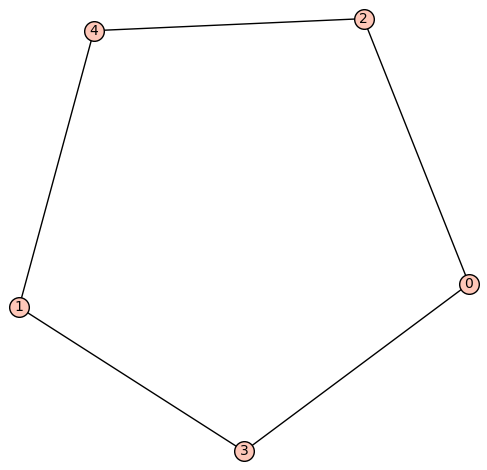
\includegraphics[width=0.5\textwidth]{sb_min_example1.png} % 0.5 pomeni pol širine strani
    \caption{Graf tipa (SB) na 5 vozliščih}
    
\end{figure}


\begin{algorithm}
    \caption{Filtriranje grafov tipa (SB)}
    \begin{algorithmic}[1]
    \State Odpri datoteko \texttt{'sb\_graphs.txt'} v načinu dodajanja (\texttt{"a"}).
    \State Odpri datoteko \texttt{"diam\_two\_graphs.txt"} v načinu branja (\texttt{"r"}).
    \For{\textbf{vsako} vrstico $line$ v datoteki \texttt{"diam\_two\_graphs.txt"}}
        \State $g \gets \textbf{pretvori\_v\_graf}(line)$ \Comment{Ustvari graf iz podatkov na trenutni vrstici.}
        \If{$is\_sb(g)$} \Comment{Preveri, če je graf $g$ tipa (SB).}
            \State Zapiši $line$ v datoteko \texttt{'sb\_graphs.txt'}.
        \EndIf
    \EndFor
    \State Zapri obe datoteki.
    \end{algorithmic}
\end{algorithm}

Z zadnjo kodo še preverimo, koliko je grafov tipa (SB) za posamezen $n$ (število vozlišč), manjši ali enak 10.
Rezultati so prikazani spodaj.



\begin{algorithm}
    \caption{Preštevanje grafov tipa (SB) z različnim številom vozlišč}
    \begin{algorithmic}[1]
    \State counter $\gets$ [0, 0, 0, \dots, 0] \Comment{ (seznam s 11 ničlami, za štetje grafov z različnim številom vozlišč)}
    \State \textbf{Odpri datoteko $'sb\_graphs\_g6.txt'$}
    \For {vsako vrstico $line$ v datoteki}
        \State $g \gets \textbf{pretvori\_v\_graf}(line)$ \Comment{ (ustvarimo graf iz vrstice)}
        \State counter[\text{len}(g.\text{vertices}())] $\gets$ counter[\text{len}(g.\text{vertices}())] + 1
    \EndFor
    \State \textbf{Izpis rezultatov:}
    \For {vsak i od 0 do 10}
        \State izpiši "Število grafov tipa (SB) z $i$ vozlišči: counter[i] "
    \EndFor
    \end{algorithmic}
 \end{algorithm}

 \begin{table}[h!]
    \centering
    \begin{tabular}{|c|c|}
    \hline
    \textbf{n (število vozlišč)} & \textbf{Število grafov tipa (SB)} \\
    \hline
    0 & 0 \\
    1 & 0 \\
    2 & 0 \\
    3 & 0 \\
    4 & 0 \\
    5 & 2 \\
    6 & 11 \\
    7 & 116\\
    8 & 1688\\
    9 & 43420 \\
    10 & 2079097 \\
    \hline
    \end{tabular}
    \caption{Tabela števila grafov tipa (SB) glede na število vozlišč}
    \end{table}

\section{Naloga 2}

Namen te naloge je naključno konstruirati grafe tipa (SB) za večje $n$.
Ideja je, da to storimo preko konstrukcije prej opisanih množic iz particije vozlišč.
Funkcija \emph{generate\_random\_sb} vzame dva argumenta; prvi je željeno število 
vozlišč, drugi pa utež, ki določi kolikšna je verjetnost povezav. Nato za začetek 
v vsako izmed petih množic iz particije razporedi eno vozlišče, ostale pa dodaja v množice 
$A_1$, $A_2$ in $A^*$ tako, da so ustrezno povezani z ostalimi skupinami za premer $2$.

Koda je dostopna v datoteki \textit{sb\_random\_alternate.py}.


\section{Naloga 3}

Želimo pridobiti tudi nov graf tipa (SB) iz danega grafa tipa (SB) tako, 
da naredimo nekaj manjših naključnih modifikacij (npr. dodajanje/odvzemanje 
vozlišč/povezav). 
\\
Koda je dostopna v datoteki \textit{random\_modify\_SB\_graph.py} na GitHubu, zaradi 
dolžine pa je zapisana le glavna ideja programa. 
\\Funkcija \textit{random\_modify\_sb\_graph} kot argument vzame graf tipa (SB) in 
ga najprej shrani (kot varovalo za kasneje, če naključne spremembe ne dajo 
grafa tipa (SB)). Zapiše particijo vozlišč in se odloči za naključno število 
naključnih sprememb iz nabora. Te spremembe so same po sebi lahke za sprogramirati, paziti 
je treba zgolj, da ne prihaja do kakšnih neželenih struktur (samozanke ...). Število sprememb je na začetku kolikor toliko majhno, da ne tvegamo,
da bi graf preveč spremenili iz tipa (SB). Program izvede te spremembe in preveri ali nov graf ustreza tipu (SB).
V kolikor ne, se postopek na takšnem grafu nadaljuje do tisočkrat, kasneje pa 
spet začnemo z originalnim grafom, ker bi bil novi graf lahko že precej degeneriran.
\\
Funkcijo sva stestirala na približno 5000 primerih, pri čemer je za $n$ blizu $30$ postopek 
v okoli $95 \%$ primerov vrnil graf tipa (SB) preden je bilo izvedenih $1000$ poskusov, torej preden smo  
spet vzeli prvotni graf. Skoraj vedno, ko je bilo generiranje grafa uspešno v teh prvih $1000$ poskusih,
se je to zgodilo v prvih $5$ poskusih, kar potrjuje smiselnost zaustavitvenega pogoja z \emph{while} zanko.
Sklepava, da so namreč bili grafi potem že zelo 'oddaljeni' od tipa (SB). Za velike $n$ je bil pri teh neuspešnih 
poskusih verjetno največkrat problem, da se je povečal premer grafa.

\section{Naloga 4}


\begin{figure}[h!]
    \centering
    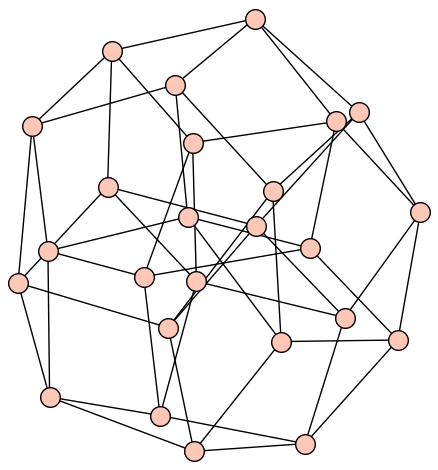
\includegraphics[width=0.5\textwidth]{sb_min_cartesian_example.png} % 0.5 pomeni pol širine strani
    \caption{Kartezični produkt grafa s slike 2 s samim seboj}
    
\end{figure}

V datoteki \emph{sb\_filter\_n.py} sva najprej prefiltrirala vse grafe tipa (SB) na do $10$ vozliščih 
v dve skupini: tiste z $8$ vozlišči ali manj in na tiste z $9$ ali $10$ vozlišči. Razlog za to je, da brute-force metoda 
za računanje dominacijskih števil vseh kartezičnih produktov grafov na do $8$ vozliščih vzame približno $11$ ur, z grafi na $9$ in $10$ vozliščih pa bi to 
že postalo časovno neizvedljivo za najine možnosti. Za izračun dominacijskih števil vseh kartezičnih 
produktov grafov na do $8$ vozliščih sva uporabila kodo \emph{sb\_domination\_brute\_force\_lower}. Vsa ta dominacijska števila sva shranila 
v datoteko \emph{sb\_cartesian\_products\_dominating\_numbers\_below\_9.txt} v mapi \emph{Podatki}.
Datoteka za vsako dominacijsko število shranjuje tudi izvorna (SB) grafa.
Predvidevava, da bi bila z vključitvijo grafov na več vozliščih dominacijska števila še večja, 
zato sklepava, da je najnižja vrednost $5$, ki jo zavzamejo $3$ kartezični produkti dveh grafov tipa (SB).
Spodnja tabela prikazuje razporeditev števila kartezičnih produktov glede na dominacijsko število.

\begin{table}[h!]
    \centering
    \begin{tabular}{|c|c|}
        \hline
        Dominacijsko število & Število grafov \\ \hline
        5 & 3 \\ \hline
        6 & 586 \\ \hline
        7 & 11339 \\ \hline
        8 & 605061 \\ \hline
        9 & 722506 \\ \hline
        10 & 307143 \\ \hline
        11 & 4992 \\ \hline
    \end{tabular}
    \caption{Razporeditev omenjenih kartezičnih produktov glede na dominacijsko število.}
\end{table}

To prikazuje tudi naslednji histogram. Skala je logaritemska.

\begin{figure}[h!]
    \centering
    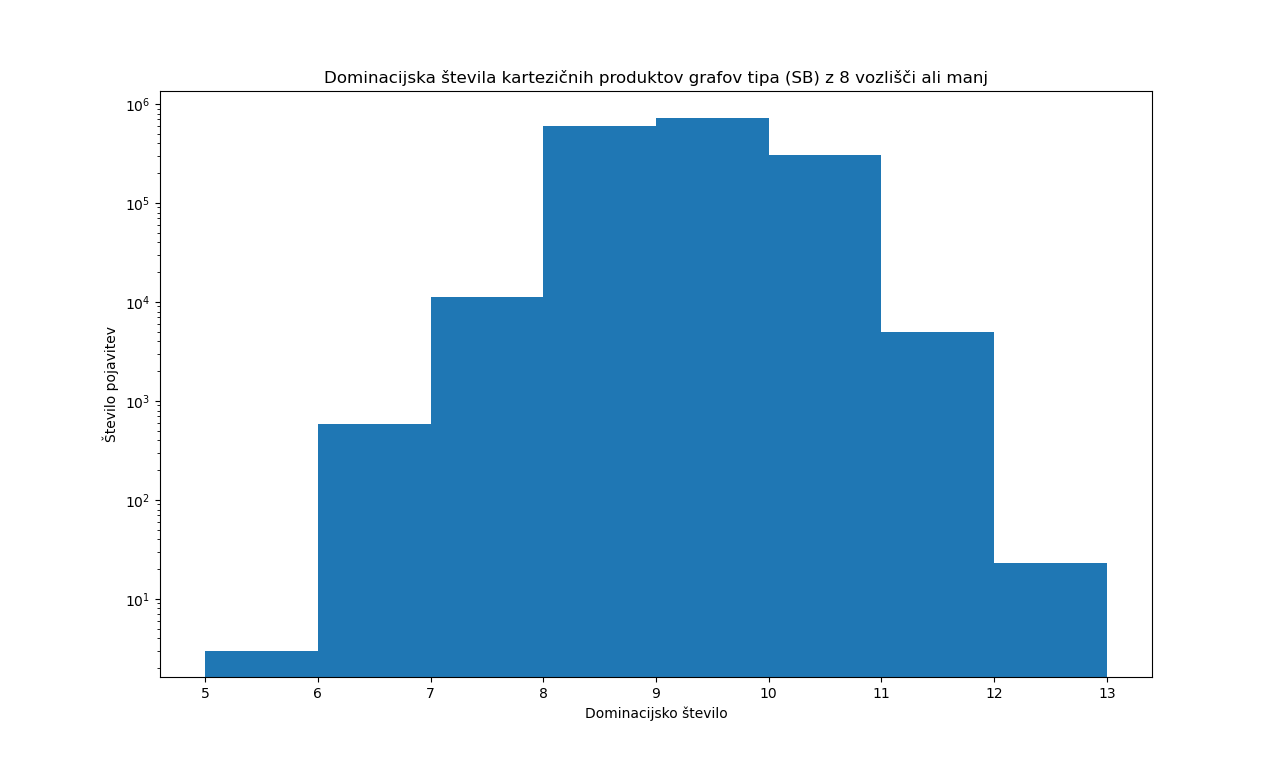
\includegraphics[width=\textwidth]{dominacijska_spodnja.png} % 0.5 pomeni pol širine strani
    
\end{figure}

Kot sva že omenila, nisva mogla poiskati vseh dominacijskih števil, zato sva za ugotavljanje zgornje meje vzela 
$10000$ naključnih kartezičnih produktov grafov tipa (SB) na $10$ vozliščih brez ponavljanja. Koda za to se nahaja 
v datoteki \emph{sb\_domination\_sampling\_upper.py}, rezultati pa v \emph{sb\_cartesian\_products\_dominating\_numbers\_upper\_sampled.txt}.
Sklepava, da je najvišje dominacijsko število kartezičnega produkta dveh grafov tipa (SB) na do $10$ vozliščih enako $14$.


\begin{table}[h!]
    \centering
    \begin{tabular}{|c|c|}
        \hline
        Dominacijsko število & Število grafov \\ \hline
        10 & 889 \\ \hline
        11 & 2646 \\ \hline
        12 & 5289 \\ \hline
        13 & 1129 \\ \hline
        14 & 46 \\ \hline
    \end{tabular}
    \caption{Razporeditev omenjenih večjih kartezičnih produktov glede na dominacijsko število.}
\end{table}

\begin{figure}[h!]
    \centering
    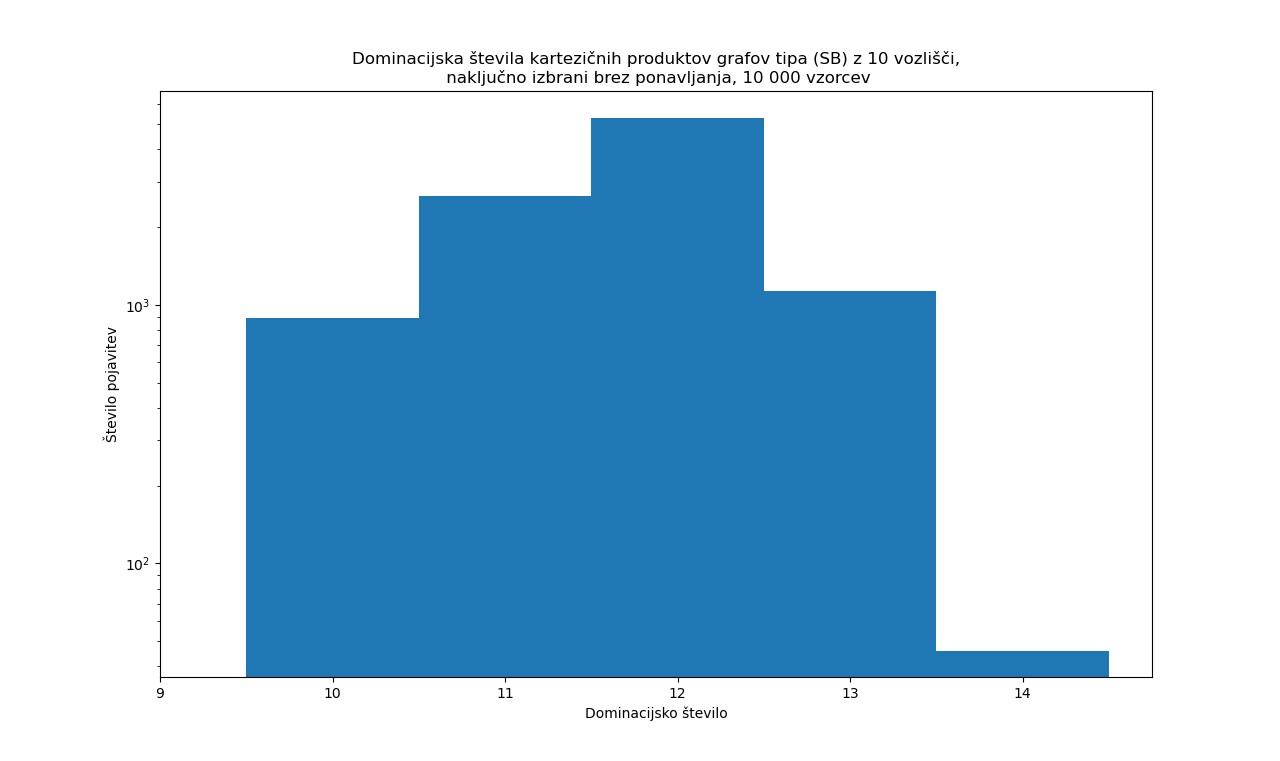
\includegraphics[width=\textwidth]{dominacijska_zgornja.png} % 0.5 pomeni pol širine strani
    
\end{figure}

\end{document}
